\section{Clustering}

\newcommand{\clusterplot}[1]{
    \begin{tikzpicture}
        \begin{axis}[
            height=6cm,
            width=6cm,
            xmajorticks=false,
            ymajorticks=false,
            xlabel=$x_1$,
            ylabel=$x_2$,
        ]
            \ifnum#1=0
                \addplot[
                    only marks,
                    mark=*,
                    blue,
                    opacity=0.5
                ] table [
                    col sep=comma,
                    x=x,
                    y=y
                ]{data/clusterdata.csv};
            \fi
            \ifnum#1=1
                \addplot[
                    only marks,
                    mark=*,
                    blue,
                    opacity=0.5
                ] table [
                    col sep=comma,
                    x=x,
                    y=y,
                    discard if not={c}{0.0}
                ]{data/clusterdata.csv};

                \addplot[
                    only marks,
                    mark=*,
                    green,
                    opacity=0.5
                ] table [
                    col sep=comma,
                    x=x,
                    y=y,
                    discard if not={c}{1.0}
                ]{data/clusterdata.csv};

                \addplot[
                    only marks,
                    mark=*,
                    red,
                    opacity=0.5
                ] table [
                    col sep=comma,
                    x=x,
                    y=y,
                    discard if not={c}{2.0}
                ]{data/clusterdata.csv};
            \fi
        \end{axis}
    \end{tikzpicture}
}

\newsavebox{\unclusteredbox}
\sbox{\unclusteredbox}{
    \clusterplot{0}
}
\newsavebox{\clusteredbox}
\sbox{\clusteredbox}{
    \clusterplot{1}
}

\begin{frame}{Clustering: Background}
    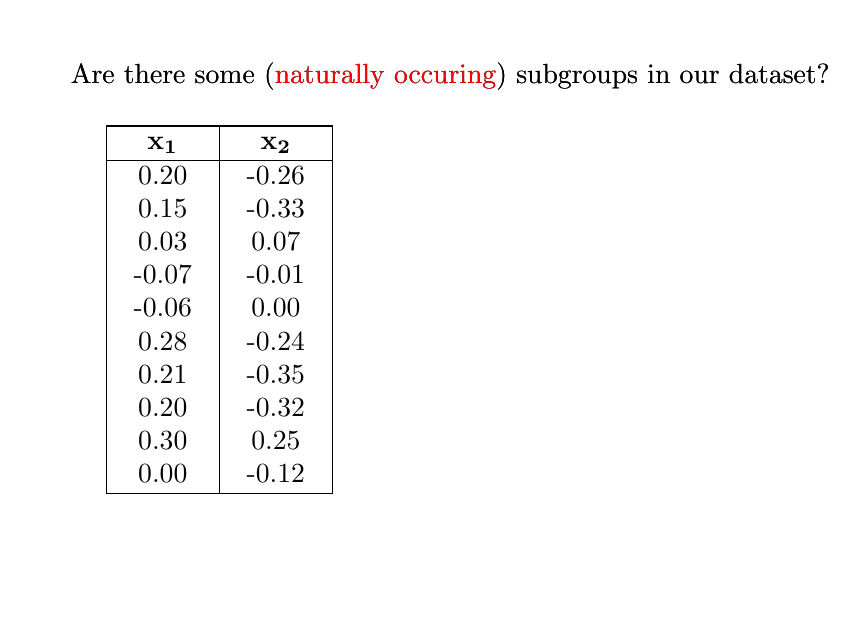
\begin{tikzpicture}
        \node[] at (-5.25, 3.5) {};
        \node[] at (-5.25, -3.5) {};

        \visible<1-4>{
            \node[] at (0, 3) {
                Are there some (naturally occuring) subgroups in our dataset?
            };
        }
        \visible<2-5>{
            \node[anchor=north west] at (-4.5, 2.5) {
                \begin{tabular}{|>{\centering\arraybackslash}p{1cm}|>{\centering\arraybackslash}p{1cm}|}
                    \hline
                    $\mathbf{x_1}$ & $\mathbf{x_2}$ \\
                    \hline
                    0.20&-0.26\\
                    0.15&-0.33\\
                    0.03&0.07\\
                    -0.07&-0.01\\
                    -0.06&0.00\\
                    0.28&-0.24\\
                    0.21&-0.35\\
                    0.20&-0.32\\
                    0.30&0.25\\
                    0.00&-0.12\\
                    \hline
                \end{tabular}
            };
        }
        \visible<3>{
            \node[anchor=north east] at (4.5, 2) {
                \usebox{\unclusteredbox}
            };
        }
        \visible<4-5>{
            \node[anchor=north east] at (4.5, 2) {
                \usebox{\clusteredbox}
            };
        }
        \visible<5>{
            \node[] at (0, 3) {
                Are there some (\textcolor{red}{naturally occuring}) subgroups in our dataset?
            };
        }
    \end{tikzpicture}
\end{frame}

\newcommand{\simpleclusterplot}[1]{
    \begin{tikzpicture}
        \begin{axis}[
            height=5.45cm,
            width=5.45cm,
            xmajorticks=false,
            ymajorticks=false,
            xlabel=$x_1$,
            ylabel=$x_2$
        ]
            \ifnum#1=0
                \addplot[
                    only marks,
                    blue,
                    opacity=0.5
                ] coordinates {
                    (1, 1)
                    (1.5, 1)
                    (1.25, 1.25)
                    (-1, 1)
                    (-1.5, 1)
                    (-1.25, 1.25)
                    (0.25, 0.0)
                    (-0.25, 0.0)
                    (0, -0.25)
                };
            \fi
            \ifnum#1=1
                \addplot[
                    only marks,
                    blue,
                    opacity=0.5
                ] coordinates {
                    (1, 1)
                    (1.5, 1)
                    (1.25, 1.25)
                };
                \addplot[
                    only marks,
                    green,
                    opacity=0.5
                ] coordinates {
                    (-1, 1)
                    (-1.5, 1)
                    (-1.25, 1.25)
                };
                \addplot[
                    only marks,
                    red,
                    opacity=0.5
                ] coordinates {
                    (0.25, 0.0)
                    (-0.25, 0.0)
                    (0, -0.25)
                };
            \fi
            \ifnum#1=2
                \addplot[
                    only marks,
                    blue,
                    opacity=0.5
                ] coordinates {
                    (1, 1)
                    (-1, 1)
                    (0.25, 0.0)
                };
                \addplot[
                    only marks,
                    green,
                    opacity=0.5
                ] coordinates {
                    (-1.5, 1)
                    (1.5, 1)
                    (-0.25, 0.0)
                };
                \addplot[
                    only marks,
                    red,
                    opacity=0.5
                ] coordinates {
                    (0, -0.25)
                    (-1.25, 1.25)
                    (1.25, 1.25)
                };
            \fi
            \ifnum#1=3
                \addplot[
                    only marks,
                    blue,
                    opacity=0.5
                ] coordinates {
                    (1, 1)
                    (1.5, 1)
                    (1.25, 1.25)
                };
                \addplot[
                    only marks,
                    green!25,
                    opacity=0.5
                ] coordinates {
                    (-1, 1)
                    (-1.5, 1)
                    (-1.25, 1.25)
                };
                \addplot[
                    only marks,
                    red!25,
                    opacity=0.5
                ] coordinates {
                    (0.25, 0.0)
                    (-0.25, 0.0)
                    (0, -0.25)
                };
            \fi
            \ifnum#1=4
                \addplot[
                    only marks,
                    blue,
                    opacity=0.5
                ] coordinates {
                    (1, 1)
                    (1.5, 1)
                };
                \addplot[
                    only marks,
                    blue!25,
                    opacity=0.5
                ] coordinates {
                    (1.25, 1.25)
                };
                \addplot[
                    only marks,
                    green!25,
                    opacity=0.5
                ] coordinates {
                    (-1, 1)
                    (-1.5, 1)
                    (-1.25, 1.25)
                };
                \addplot[
                    only marks,
                    red!25,
                    opacity=0.5
                ] coordinates {
                    (0.25, 0.0)
                    (-0.25, 0.0)
                    (0, -0.25)
                };
            \fi
            \ifnum#1=5
                \addplot[
                    only marks,
                    blue,
                    opacity=0.5
                ] coordinates {
                    (1, 1)
                    (1.25, 1.25)
                };
                \addplot[
                    only marks,
                    blue!25,
                    opacity=0.5
                ] coordinates {
                    (1.5, 1)
                };
                \addplot[
                    only marks,
                    green!25,
                    opacity=0.5
                ] coordinates {
                    (-1, 1)
                    (-1.5, 1)
                    (-1.25, 1.25)
                };
                \addplot[
                    only marks,
                    red!25,
                    opacity=0.5
                ] coordinates {
                    (0.25, 0.0)
                    (-0.25, 0.0)
                    (0, -0.25)
                };
            \fi
            \ifnum#1=6
                \addplot[
                    only marks,
                    blue,
                    opacity=0.5
                ] coordinates {
                    (1.25, 1.25)
                    (1.5, 1)
                };
                \addplot[
                    only marks,
                    blue!25,
                    opacity=0.5
                ] coordinates {
                    (1, 1)
                };
                \addplot[
                    only marks,
                    green!25,
                    opacity=0.5
                ] coordinates {
                    (-1, 1)
                    (-1.5, 1)
                    (-1.25, 1.25)
                };
                \addplot[
                    only marks,
                    red!25,
                    opacity=0.5
                ] coordinates {
                    (0.25, 0.0)
                    (-0.25, 0.0)
                    (0, -0.25)
                };
            \fi
        \end{axis}
    \end{tikzpicture}
}

\newsavebox{\simpleunclustered}
\sbox{\simpleunclustered}{
    \simpleclusterplot{0}
}
\newsavebox{\simpleclustered}
\sbox{\simpleclustered}{
    \simpleclusterplot{1}
}
\newsavebox{\simplebad}
\sbox{\simplebad}{
    \simpleclusterplot{2}
}
\newsavebox{\simplesingle}
\sbox{\simplesingle}{
    \simpleclusterplot{3}
}
\newsavebox{\simplefirst}
\sbox{\simplefirst}{
    \simpleclusterplot{4}
}
\newsavebox{\simplesecond}
\sbox{\simplesecond}{
    \simpleclusterplot{5}
}
\newsavebox{\simplethird}
\sbox{\simplethird}{
    \simpleclusterplot{6}
}

\begin{frame}{K-means clustering}
    \begin{tikzpicture}
        \node[] at (-5.25, 3.5) {};
        \node[] at (-5.25, -3.5) {};

        \visible<1-2>{
            \node[text width=10cm, align=left] at (0, -2) {
                \underline{K-means clustering}: Find $k$ clusters in the data to minimze the \textit{within-cluster variance}:
            };
        }
        \visible<1>{
            \node[] at (0, -3) {
                $\underset{C_1,...,C_k}{\mathrm{minimize}} \left( \sum\limits_{k=1}^K \dfrac{1}{|C_k|} \sum\limits_{i,i' \in C_k}  \sum\limits_{j=1}^p (x_{ij} - x_{i'j})^2 \right)$
            };
        }
        \visible<2-20>{
            \node[] at (0, -3) {
                $\alert<4-7>{\underset{C_1,...,C_k}{\mathrm{minimize}}} \left( \alert<8-9>{\sum\limits_{k=1}^K} \alert<10>{\dfrac{1}{|C_k|}} \alert<11-16>{\sum\limits_{i,i' \in C_k}} \sqrt{\alert<17-18>{\sum\limits_{j=1}^p} (x_{ij} - x_{i'j})^2} \right)$
            };
        }
        \visible<3-4>{
            \node[anchor=north east] at (4.5, 3) {
                \usebox{\simpleunclustered}
            };
        }
        \visible<3-20>{
            \node[anchor=north west] (data) at (-4.5, 3) {
                {\footnotesize
                \begin{tabular}{|>{\centering\arraybackslash}p{1cm}|>{\centering\arraybackslash}p{1cm}|}
                    \hline
                    $\mathbf{x_1}$ & $\mathbf{x_2}$ \\
                    \hline
                    \only<3-15>{1}\only<16->{\textcolor{black!25}{1}}&\only<3-15>{1}\only<16->{\textcolor{black!25}{1}}\\
                    1.5&1\\
                    1.25&1.25\\
                    \only<3-8>{-1}\only<9->{\textcolor{black!25}{-1}}&\only<3-8>{1}\only<9->{\textcolor{black!25}{1}}\\
                    \only<3-8>{-1.5}\only<9->{\textcolor{black!25}{-1.5}}&\only<3-8>{1}\only<9->{\textcolor{black!25}{1}}\\
                    \only<3-8>{-1.25}\only<9->{\textcolor{black!25}{-1.25}}&\only<3-8>{1.25}\only<9->{\textcolor{black!25}{1.25}}\\
                    \only<3-8>{0.25}\only<9->{\textcolor{black!25}{0.25}}&\only<3-8>{0}\only<9->{\textcolor{black!25}{0}}\\
                    \only<3-8>{-0.25}\only<9->{\textcolor{black!25}{-0.25}}&\only<3-8>{0}\only<9->{\textcolor{black!25}{0}}\\
                    \only<3-8>{0}\only<9->{\textcolor{black!25}{0}}&\only<3-8>{-0.25}\only<9->{\textcolor{black!25}{-0.25}}\\
                    \hline
                \end{tabular}
                }
            };
        }
        \visible<5,7-8>{
            \node[anchor=north east] at (4.5, 3) {
                \usebox{\simpleclustered}
            };
            \node[anchor=west, text=blue, font=\footnotesize\selectfont] at ($ (data.east) + (0, 1.35) $) {
                $C_1$
            };
            \node[anchor=west, text=blue, font=\footnotesize\selectfont] at ($ (data.east) + (0, 0.97) $) {
                $C_1$
            };
            \node[anchor=west, text=blue, font=\footnotesize\selectfont] at ($ (data.east) + (0, 0.59) $) {
                $C_1$
            };
            \node[anchor=west, text=green, font=\footnotesize\selectfont] at ($ (data.east) + (0, 0.21) $) {
                $C_2$
            };
            \node[anchor=west, text=green, font=\footnotesize\selectfont] at ($ (data.east) + (0, -0.17) $) {
                $C_2$
            };
            \node[anchor=west, text=green, font=\footnotesize\selectfont] at ($ (data.east) + (0, -0.55) $) {
                $C_2$
            };
            \node[anchor=west, text=red, font=\footnotesize\selectfont] at ($ (data.east) + (0, -0.93) $) {
                $C_3$
            };
            \node[anchor=west, text=red, font=\footnotesize\selectfont] at ($ (data.east) + (0, -1.31) $) {
                $C_3$
            };
            \node[anchor=west, text=red, font=\footnotesize\selectfont] at ($ (data.east) + (0, -1.69) $) {
                $C_3$
            };
        }

        \visible<6>{
            \node[anchor=north east] at (4.5, 3) {
                \usebox{\simplebad}
            };
            \node[anchor=west, text=blue, font=\footnotesize\selectfont] at ($ (data.east) + (0, 1.35) $) {
                $C_1$
            };
            \node[anchor=west, text=green, font=\footnotesize\selectfont] at ($ (data.east) + (0, 0.97) $) {
                $C_2$
            };
            \node[anchor=west, text=red, font=\footnotesize\selectfont] at ($ (data.east) + (0, 0.59) $) {
                $C_3$
            };
            \node[anchor=west, text=blue, font=\footnotesize\selectfont] at ($ (data.east) + (0, 0.21) $) {
                $C_1$
            };
            \node[anchor=west, text=green, font=\footnotesize\selectfont] at ($ (data.east) + (0, -0.17) $) {
                $C_2$
            };
            \node[anchor=west, text=red, font=\footnotesize\selectfont] at ($ (data.east) + (0, -0.55) $) {
                $C_3$
            };
            \node[anchor=west, text=blue, font=\footnotesize\selectfont] at ($ (data.east) + (0, -0.93) $) {
                $C_1$
            };
            \node[anchor=west, text=green, font=\footnotesize\selectfont] at ($ (data.east) + (0, -1.31) $) {
                $C_2$
            };
            \node[anchor=west, text=red, font=\footnotesize\selectfont] at ($ (data.east) + (0, -1.69) $) {
                $C_3$
            };
        }
        \visible<9-12>{
            \node[anchor=north east] at (4.5, 3) {
                \usebox{\simplesingle}
            };
            \node[anchor=west, text=blue, font=\footnotesize\selectfont] at ($ (data.east) + (0, 1.35) $) {
                $C_1$
            };
            \node[anchor=west, text=blue, font=\footnotesize\selectfont] at ($ (data.east) + (0, 0.97) $) {
                $C_1$
            };
            \node[anchor=west, text=blue, font=\footnotesize\selectfont] at ($ (data.east) + (0, 0.59) $) {
                $C_1$
            };
            \node[anchor=west, text=green!25, font=\footnotesize\selectfont] at ($ (data.east) + (0, 0.21) $) {
                $C_2$
            };
            \node[anchor=west, text=green!25, font=\footnotesize\selectfont] at ($ (data.east) + (0, -0.17) $) {
                $C_2$
            };
            \node[anchor=west, text=green!25, font=\footnotesize\selectfont] at ($ (data.east) + (0, -0.55) $) {
                $C_2$
            };
            \node[anchor=west, text=red!25, font=\footnotesize\selectfont] at ($ (data.east) + (0, -0.93) $) {
                $C_3$
            };
            \node[anchor=west, text=red!25, font=\footnotesize\selectfont] at ($ (data.east) + (0, -1.31) $) {
                $C_3$
            };
            \node[anchor=west, text=red!25, font=\footnotesize\selectfont] at ($ (data.east) + (0, -1.69) $) {
                $C_3$
            };
        }
        \visible<12>{
            \node[] (i) at ($ (data.west) - (0.2, 0) $) {
                $i$
            };
            \draw[-stealth] (i.north) -- ($ (i.north) + (0, 1.6) $);
            \draw[-stealth] (i.south) -- ($ (i.south) - (0, 1.6) $);
        }
        \visible<13>{
            \node[anchor=north east] at (4.5, 3) {
                \usebox{\simplefirst}
            };
            \draw[stealth-stealth] ($ (data.west) + (0, 1.35) $) -- ($ (data.west) + (-0.3, 1.35) $) -- ($ (data.west) + (-0.3, 0.97) $) -- ($ (data.west) + (0, 0.97) $);
        }
        \visible<14>{
            \node[anchor=north east] at (4.5, 3) {
                \usebox{\simplesecond}
            };
            \draw[stealth-stealth] ($ (data.west) + (0, 1.35) $) -- ($ (data.west) + (-0.3, 1.35) $) -- ($ (data.west) + (-0.3, 0.59) $) -- ($ (data.west) + (0, 0.59) $);
        }
        \visible<15>{
            \draw[stealth-stealth] ($ (data.west) + (0, 0.97) $) -- ($ (data.west) + (-0.3, 0.97) $) -- ($ (data.west) + (-0.3, 0.59) $) -- ($ (data.west) + (0, 0.59) $);
        }
        \visible<15-18>{
            \node[anchor=north east] at (4.5, 3) {
                \usebox{\simplethird}
            };
        }
        \visible<18>{
            \node[] (j) at ($ (data.north) + (0, 0.2) $) {
                j
            };
            \draw[-stealth] (j.east) -- ($ (j.east) + (1.2, 0) $);
            \draw[-stealth] (j.west) -- ($ (j.west) - (1.2, 0) $);
        }
    \end{tikzpicture}
\end{frame}
